\documentclass{article}

\usepackage[a4paper,margin=2cm]{geometry}
\usepackage{graphicx}
\usepackage{subcaption}
\usepackage{hyperref}
\usepackage{appendix}

\title{COMP30027 Assignment 1 - Report}
\date{\today}
\author{Lucas Fern (1080613)}

\begin{document}
\maketitle
\noindent Overall, the Naïve Bayes classifier implemented for this assignment achieved an accuracy of 75.9\% on the provided training data. The accuracies within individual classes varied between 42.9\% and 100\%, and the individual accuracies as read from the diagonal of the confusion matrix in figure \ref{fig: conf prop} are:
\begin{verbatim}
    Multiclass Accuracy:
        bridge: 0.429
        childs: 0.917
        downwarddog: 0.867
        mountain: 0.867
        plank: 0.667
        seatedforwardbend: 0.444
        tree: 0.667
        trianglepose: 1.000
        warrior1: 0.800
        warrior2: 0.875
\end{verbatim}

\subsection*{Question 1: Multiclass Model Evaluation}
For this question both Micro and Macro-Averaging were implemented for the multiclass precision, recall, and $F_{1}$ score. All of these scores can be easily generated from a confusion matrix containing the frequencies of each classification. A visualisation of the confusion matrix from running the model on the test data is shown in figure \ref{fig: conf freq}, and what is perhaps a more useful confusion matrix showing the proportions is presented alongside in figure \ref{fig: conf prop}.\\[2mm]
Calculating the Micro and Macro-Averaged statistics from the confusion matrix gives the following results:
\begin{verbatim}
    Multiclass Precision (Macro-Averaged):
        0.739
    Multiclass Recall (Macro-Averaged):
        0.753
    Multiclass F1 Score (Macro-Averaged):
        0.746
    Multiclass Precision (Micro-Averaged):
        0.759
    Multiclass Recall (Micro-Averaged):
        0.759
    Multiclass F1 Score (Micro-Averaged):
        0.759
\end{verbatim}
It is clear from this output that the choice of Micro vs. Macro-Averaging makes only a very small difference in this case, with the largest difference being between the Micro and Macro-Averaged precision at 2\%. It is surprising that all the micro-averaged statistics are identical, but this is simply a coincidence, and it can be seen easily from the formula for the $F_{1}$ score that when the precision and recall are identical, the $F_{1}$ score will be too:
$$F_{1} = \frac{2PR}{P + R}; \qquad \mbox{when } P = R = \alpha; \qquad F_{1} = \frac{2 \alpha^{2}}{2 \alpha} = \alpha$$ 
Apart from this, none of the results are unexpected. The Macro-Averaged scores appear to be slightly lower since the Micro-Averaging process considers the size of the class when averaging, whereas the Macro-Averaging process takes a non-weighted average of the precision and recall from each class. This means that classes which appear in large quantities in the test data - such as the mountain pose - are represented with larger weighting in the Micro-Averaged scores. In this example, the mountain pose class has an accuracy of 0.867, which is above the average accuracy, and therefore contributes significantly to increasing the Micro-Averaged precision and recall.

\begin{figure}[]
    \centering
    \caption{A visualisation of two confusion matrices for the model's classification of the testing data.}
    \label{fig: conf mats}
    \begin{subfigure}[b]{0.75\linewidth}
        \caption{Using frequencies.}
        \label{fig: conf freq}
        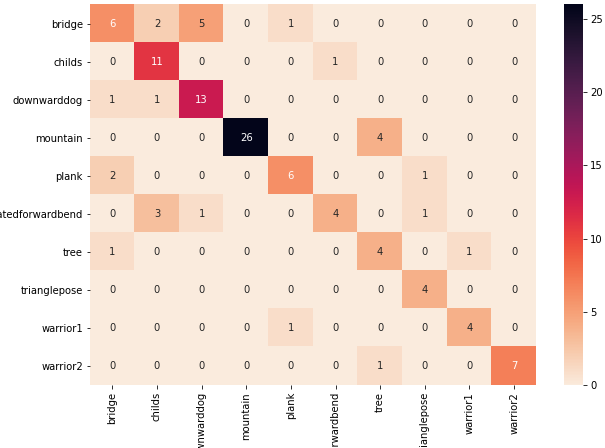
\includegraphics[width=\linewidth]{conf-frequencies.png}
    \end{subfigure}
    \par\bigskip
    \begin{subfigure}[b]{0.75\linewidth}
        \caption{Using proportions.}
        \label{fig: conf prop}
        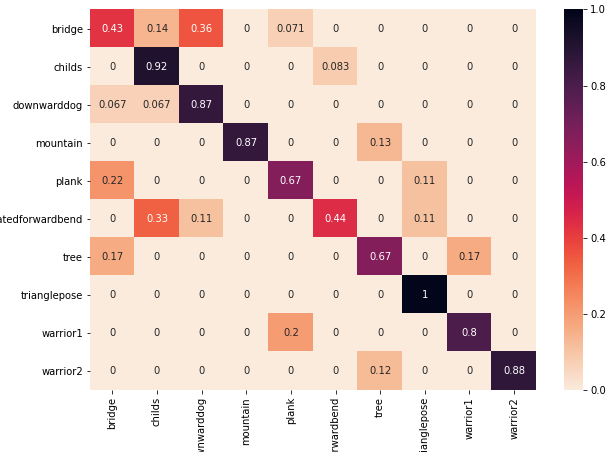
\includegraphics[width=\linewidth]{conf-proportions.png}
    \end{subfigure}
\end{figure}

\subsection*{Question 2: Gaussian Distribution Assumption}
The Gaussian Naïve Bayes classifier assumes that observations for attributes are normally distributed within each class. To check the validity of these assumptions a large amount of visualisations were generated, the most useful of which are presented below.\\[2mm]
The number of normal distributions that are fit for the Gaussian Naïve Bayes classifier is equal to the number of classes (10) times the number of attributes (22). To exhaustively check the normal assumption would be to verify it held for all of these 220 distributions. It does not.\\[2mm]
This was visualised in two ways, the prettiest and most information dense option being a scatterplot of the coordinates of a body part for all of the different poses. Marginal density plots on each of the axes allow us to assess the distribution of coordinates for each axis, for each pose. These plots for each of the body parts are shown in figure \ref{fig: scatters} from appendix \ref{app: scatters}, but we will look specifically at figures \ref{fig: head} and \ref{fig: chest} for an example. These will be used to argue that there is insufficient evidence in this data to conclude that violating the assumption of normality decreases the accuracy of classification results.\\[2mm]
Firstly, it can be observed from figure \ref{fig: conf prop} that Triangle pose was the class most accurately classified by the model, and Bridge pose was the least. Looking closely it can be seen in the marginal density plots on figures \ref{fig: head} and \ref{fig: chest} that the Triangle pose does not fit well to a Gaussian distribution, and Bridge pose does significantly better, especially in the distribution of the $x$ coordinates, where Triangle pose seems to be multimodal (which is not a property of normal distributions). We can visualise this more clearly by taking Normal QQ plots of these body part coordinates. This is shown in appendix \ref{app: QQ} figure \ref{fig: QQs}, where \ref{fig: tri head} and \ref{fig: tri chest} show convincingly that these data points from the Triangle pose data do \textit{not} follow a normal distribution. Figures \ref{fig: bridge head} and \ref{fig: bridge chest} show that the Bridge pose coordinates do fit the normal distribution better, though still not perfectly.\\[2mm]
Because the class most accurately predicted by the model shows less adherence to the normal assumption than the class worst predicted in many of the cases, there is insufficient evidence to conclude that violation of the normal assumption has a negative effect on the accuracies of the classifiers predictions.

\newpage
\appendix
\section*{Appendices}
\section{Normal QQ Plots of Body Part Coordinate Distributions}
\label{app: QQ}
\begin{figure}[h!]
    \caption{A set of QQ plots demonstrating that the Triangle pose adheres less to the Gaussian distribution assumption than the Bridge pose for some selections of body parts.}
    \label{fig: QQs}
    \centering
    \begin{subfigure}[b]{0.4\linewidth}
        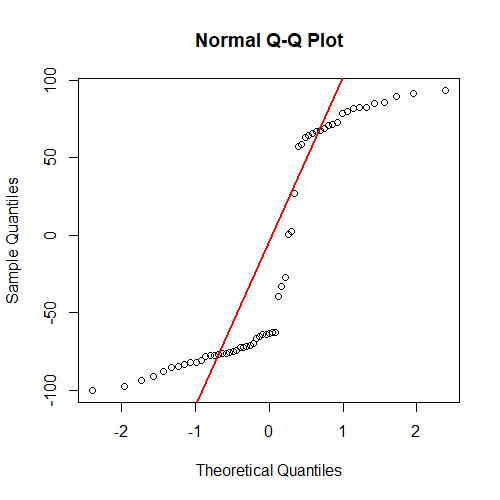
\includegraphics[width=\linewidth]{limb-distribution/triangle_qq_head_x.png}
        \caption{QQ Plot for $x$ coordinates of heads from Triangle poses.}
        \label{fig: tri head}
    \end{subfigure}
    \hspace{1cm}
    \begin{subfigure}[b]{0.4\linewidth}
        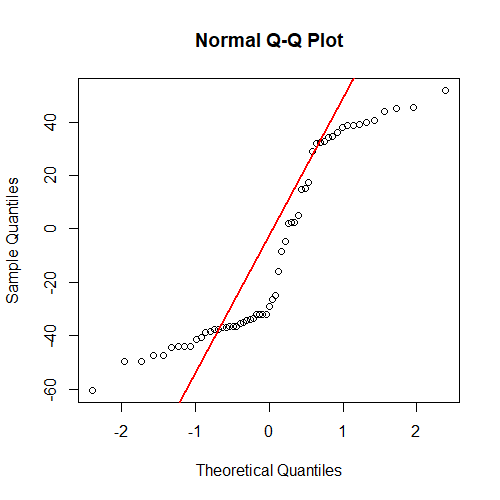
\includegraphics[width=\linewidth]{limb-distribution/triangle_qq_chest_x.png}
        \caption{QQ Plot for $x$ coordinates of chests from Triangle poses.}
        \label{fig: tri chest}
    \end{subfigure}
    \begin{subfigure}[b]{0.4\linewidth}
        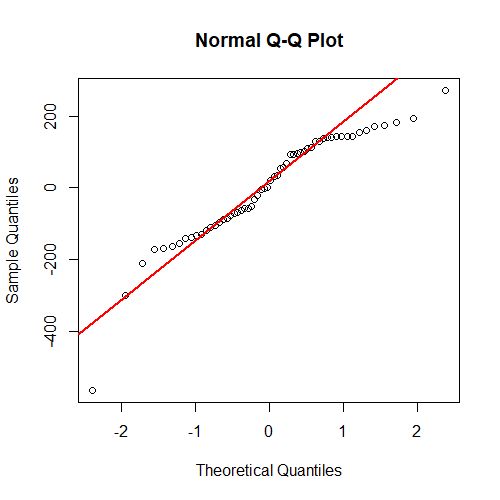
\includegraphics[width=\linewidth]{limb-distribution/bridge_qq_head_x.png}
        \caption{QQ Plot for $x$ coordinates of heads from Bridge poses.}
        \label{fig: bridge head}
    \end{subfigure}
    \hspace{1cm}
    \begin{subfigure}[b]{0.4\linewidth}
        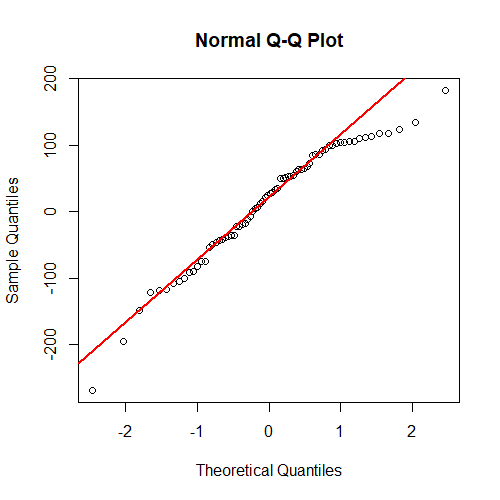
\includegraphics[width=\linewidth]{limb-distribution/bridge_qq_chest_x.png}
        \caption{QQ Plot for $x$ coordinates of chests from Bridge poses.}
        \label{fig: bridge chest}
    \end{subfigure}
\end{figure}

\newpage
\section{Body Part Distribution Scatterplots}
\label{app: scatters}
\begin{figure}[!h]
    \caption{Scatterplots of all body part coordinates in training data with marginal distributions. Coloured by true pose. (You can ignore most of these, they are just included for completeness and because they look nice \url{:)})}
    \label{fig: scatters}
    \begin{subfigure}[t]{\linewidth}
        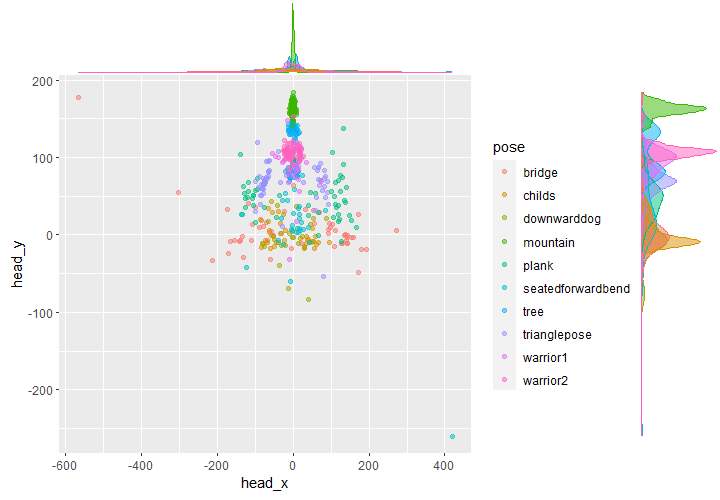
\includegraphics[width=0.9\linewidth]{limb-distribution/head.png}
        \caption{The distribution of head coordinates with marginal density plots.}
        \label{fig: head}
    \end{subfigure}
    \begin{subfigure}[t]{\linewidth}
        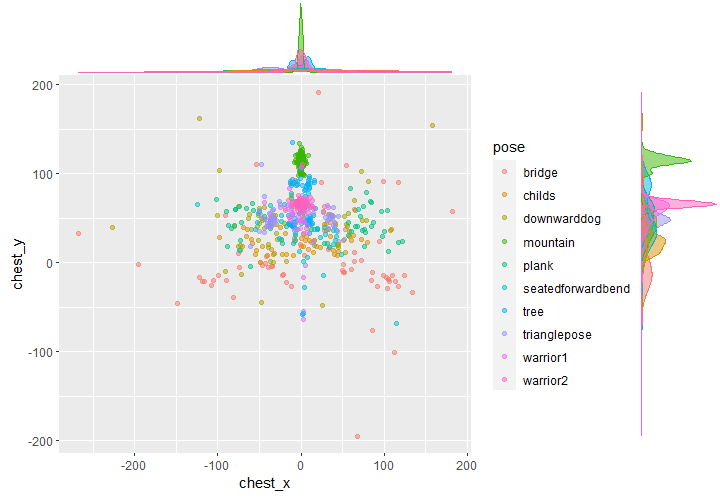
\includegraphics[width=0.9\linewidth]{limb-distribution/chest.png}
        \caption{The distribution of chest coordinates with marginal density plots.}
        \label{fig: chest}
    \end{subfigure}  
\end{figure}
\begin{figure}\ContinuedFloat
    \begin{subfigure}[b]{\linewidth}
        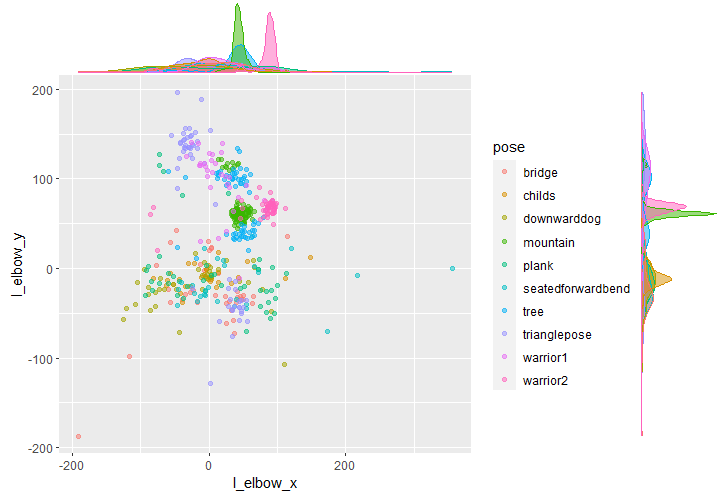
\includegraphics[width=0.9\linewidth]{limb-distribution/l_elbow.png}
        \caption{The distribution of left elbow coordinates with marginal density plots.}
        \label{fig: l_elbow}
    \end{subfigure}
    \begin{subfigure}[b]{\linewidth}
        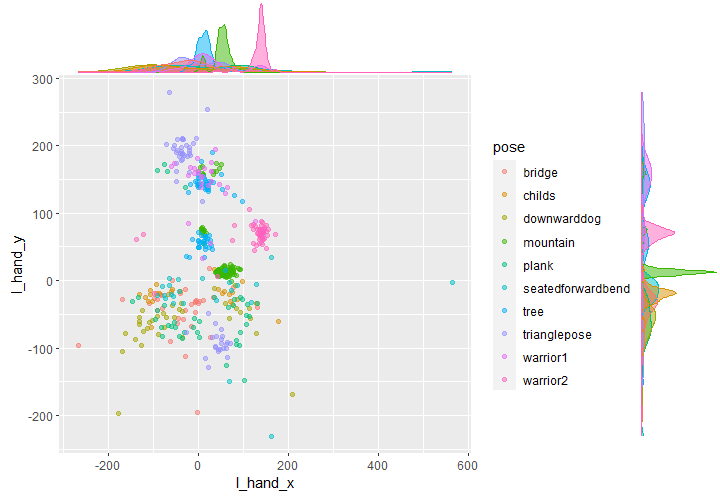
\includegraphics[width=0.9\linewidth]{limb-distribution/l_hand.png}
        \caption{The distribution of left hand coordinates with marginal density plots.}
        \label{fig: l_hand}
    \end{subfigure}
\end{figure}
\begin{figure}\ContinuedFloat
    \begin{subfigure}[b]{\linewidth}
        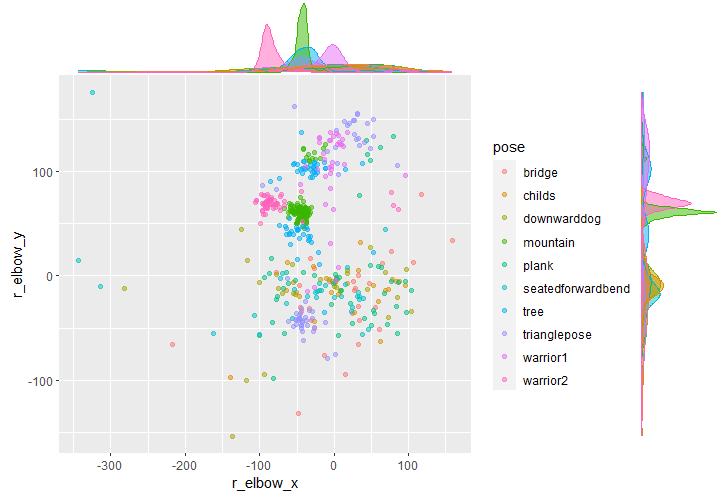
\includegraphics[width=0.9\linewidth]{limb-distribution/r_elbow.png}
        \caption{The distribution of right elbow coordinates with marginal density plots.}
        \label{fig: r_elbow}
    \end{subfigure}
    \begin{subfigure}[b]{\linewidth}
        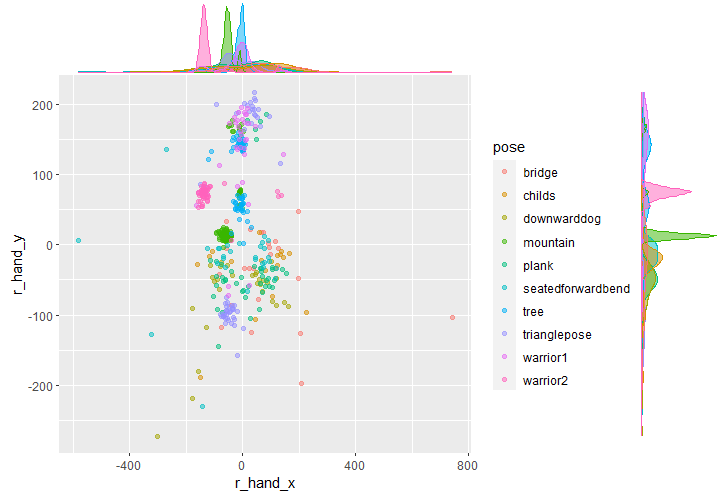
\includegraphics[width=0.9\linewidth]{limb-distribution/r_hand.png}
        \caption{The distribution of right hand coordinates with marginal density plots.}
        \label{fig: r_hand}
    \end{subfigure}
\end{figure}
\begin{figure}\ContinuedFloat
    \begin{subfigure}[b]{\linewidth}
        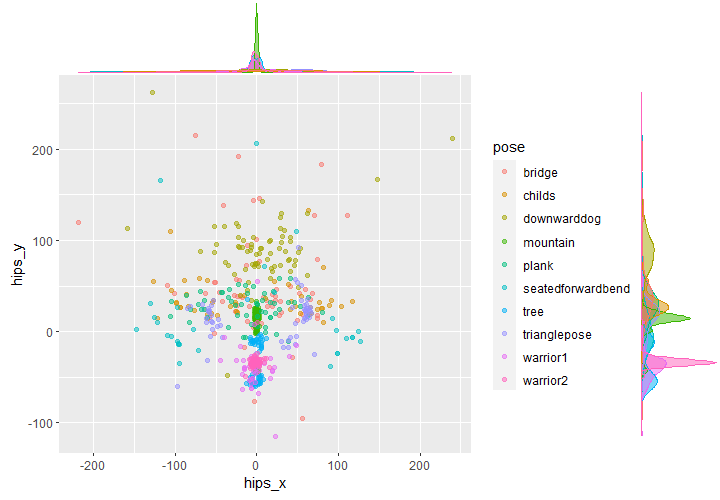
\includegraphics[width=0.9\linewidth]{limb-distribution/hips.png}
        \caption{The distribution of hip coordinates with marginal density plots.}
        \label{fig: hips}
    \end{subfigure}
    \begin{subfigure}[b]{\linewidth}
        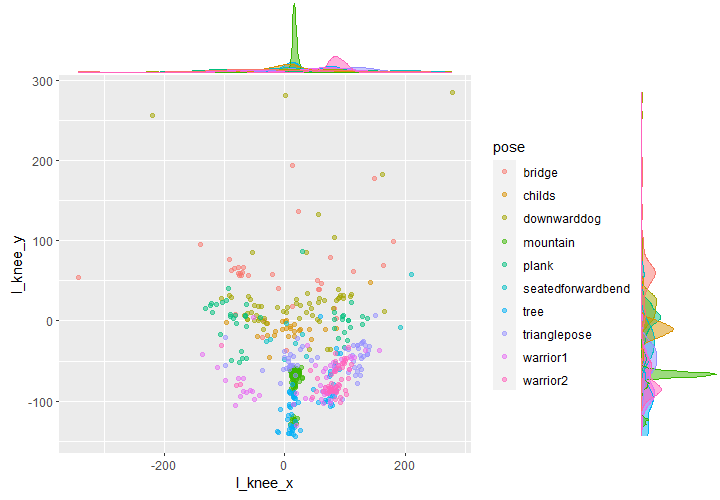
\includegraphics[width=0.9\linewidth]{limb-distribution/l_knee.png}
        \caption{The distribution of left knee coordinates with marginal density plots.}
        \label{fig: l_knee}
    \end{subfigure}
\end{figure}
\begin{figure}\ContinuedFloat
    \begin{subfigure}[b]{\linewidth}
        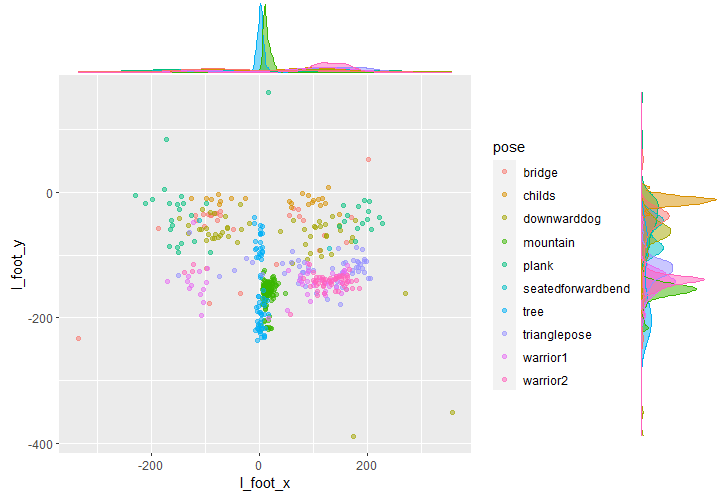
\includegraphics[width=0.9\linewidth]{limb-distribution/l_foot.png}
        \caption{The distribution of left foot coordinates with marginal density plots.}
        \label{fig: l_foot}
    \end{subfigure}
    \begin{subfigure}[b]{\linewidth}
        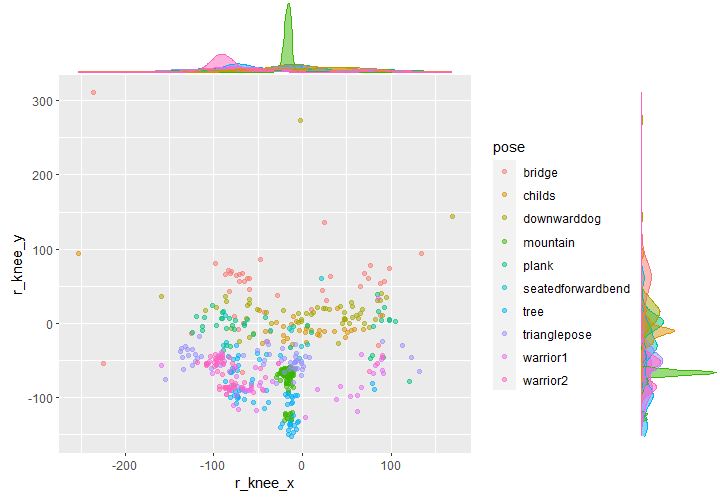
\includegraphics[width=0.9\linewidth]{limb-distribution/r_knee.png}
        \caption{The distribution of right knee coordinates with marginal density plots.}
        \label{fig: r_knee}
    \end{subfigure}
\end{figure}
\begin{figure}\ContinuedFloat
    \begin{subfigure}[b]{\linewidth}
        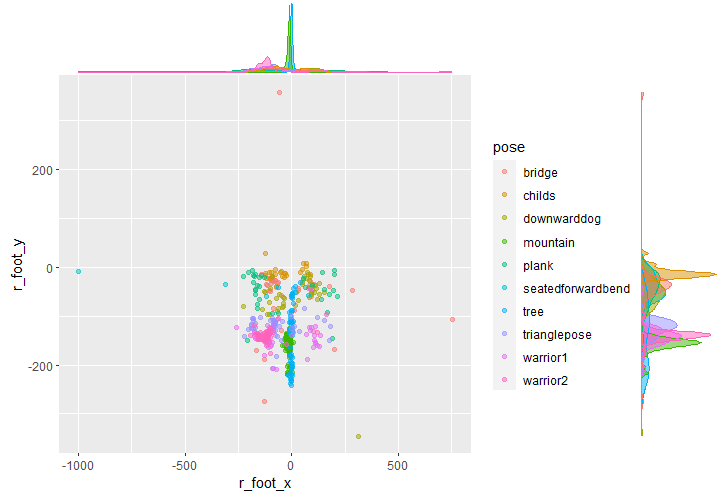
\includegraphics[width=0.9\linewidth]{limb-distribution/r_foot.png}
        \caption{The distribution of right foot coordinates with marginal density plots.}
        \label{fig: r_foot}
    \end{subfigure}
\end{figure}



\end{document}